\begin{frame}{Multiclass Classification I: Loss Function}

\vspace{0.1in}
The standard cross entropy loss is defined to be
\begin{equation}
    \label{eq:xentropy}
    \ell(W;(\x,y)) = - \log \frac {\exp(-\trans\w_y \x)}{\sum_{j=1}^k \exp(-\trans \w_j \x)}
\vspace{-0.1in}
\end{equation}
where
\begin{itemize}
    %\item $(\x, y)$ is an input data point
    \item $\x \in \R^d$ is an input feature vector
    \item $y \in \{1, 2, ..., k\}$ is the input class label
    \item $\w_i \in \R^d$ is the parameter vector for class $i$
    \item $W = (\w_1, \w_2, ..., \w_k) \in \R^{d\times k}$ is the parameter matrix
\end{itemize}

\uncover<2>{
\vspace{0.2in}
    \textbf{Goal:} Approximate the optimal parameter matrix
\begin{equation}
    W^* = \argmin_{W} \E \ell(W; (\x,y))
    .
\end{equation}
}
\end{frame}

%%%%%%%%%%%%%%%%%%%%%%%%%%%%%%%%%%%%%%%%%%%%%%%%%%%%%%%%%%%%%%%%%%%%%%%%%%%%%%%%
\begin{frame}{Multiclass Classification II: SGD}

Approximate $W^*$ using \emph{stochastic gradient descent} (SGD):
\begin{equation}
    W_{t+1} = W_t - \eta \nabla \ell(W_t, (\x_t, y_t))
\end{equation}
where $\eta$ is the step size/learning rate.

%\vspace{0.2in}
%As $t \to \infty$, $W_t \to W^*$.

%\vspace{0.2in}
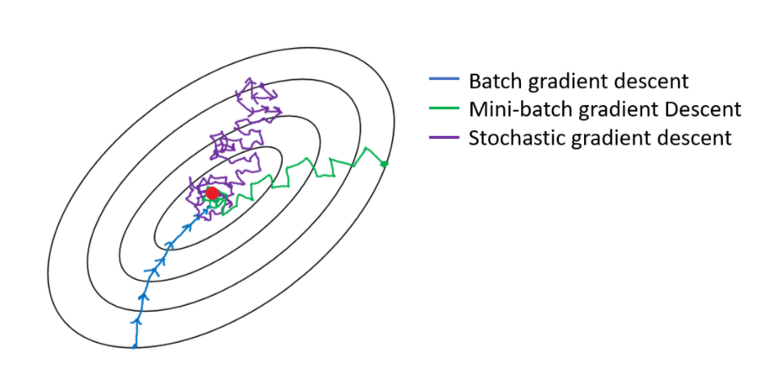
\includegraphics[height=2in]{img/sgd}

{\tiny
Image Source: \url{https://sweta-nit.medium.com/batch-mini-batch-and-stochastic-gradient-descent-e9bc4cacd461}
}
\end{frame}

%%%%%%%%%%%%%%%%%%%%%%%%%%%%%%%%%%%%%%%%%%%%%%%%%%%%%%%%%%%%%%%%%%%%%%%%%%%%%%%%
\ignore{
\begin{frame}{SGD}
We let $\theta^{(t)}$ denote the parameter value at iteration $t$,
and $\eta : \mathbb R$ be the step size.
Let $\nu_t$ be a noisy gradient of $f$ satisfying
\begin{equation}
    \E[\nu_t | \theta^{(t)}] = \nabla f(\theta^{(t)}).
\end{equation}
Then the parameter update for step $t$ is defined to be
\begin{equation}
    \theta^{(t+1)} = \theta^{(t)} - \eta \nabla \nu_t
    .
\end{equation}
When using parameter averaging, the final model parameters are defined to be
\begin{equation}
    \bar\theta = \frac1T \sum_{i=1}^T \theta^{(t)}
    .
\end{equation}
\end{frame}
}
%%%%%%%%%%%%%%%%%%%%%%%%%%%%%%%%%%%%%%%%%%%%%%%%%%%%%%%%%%%%%%%%%%%%%%%%%%%%%%%%
\ignore{
\begin{frame}{Multiclass Classification II: Objectives}

The \emph{true loss} is defined to be
\begin{equation}
    L_D(W) = \E_{(\x,y)\sim D} \ell(W; (\x, y))
\end{equation}
where $D$ is the unknown data distribution.

\vspace{0.2in}
The \emph{optimal parameter matrix} is 
\begin{equation}
    W^* = \argmin_{W} L_D(W)
\end{equation}

\end{frame}
}
